% !TEX root = ../main.tex
\section{Description of the Sample Application}
\label{sec:descr-sample-appl}

To illustrate the development and analysis process of a design using the previously described 
statechart semantics, we will discuss a quadrotor helicopter or quadrotor application similar to 
the one presented by Syriani et al.~\cite{Syriani_2019}. The application will focus on the incremental 
design of some of the drone's required functionality.
The \SonChange{model constructed}{constructed model} must obey statechart refinement rules that are proven within the Rodin tool.
The structure of the statechart for this model at each subsequent abstraction level \SonChange{restrict farther}{restricts further the} 
development of the model to refinements that obey the rules. This will allow us to prove properties 
of the model in a very strategic fashion, as properties proven of early abstraction levels 
are preserved in later refinements.

The first abstraction of the model shown in \SonChange{figure}{Figure}~\ref{fig:drone1} captures the basic 
functionality of the drone. The model's initial state is |OFF| and as a result of the |on| and 
|toTakeoff| external triggers it transitions to the |START| and |OPERATIONAL| states 
respectively\footnote{Transitions in Figures~\ref{fig:drone1}--\ref{fig:drone4} are labeled with trigger names
(e.g. toTakeoff, toFly) not with event names as it is in \UMLB.}. 
The drone reacts to the |off| external trigger by shutting down and subsequently transitioning to the |OFF| state.
Within the |OPERATIONAL| state the drone will transition to |FLY|, |DESCEND| or |LANDED| 
state after the internal trigger |toFly|, |toLand| or |landed| is raised, respectively. 
In this abstraction, these internal triggers are raised non-deterministically 
in the system by functionality not currently defined.
As additional details are incorporated into the model in later refinements some of that non-determinism is 
removed and replaced by transitions with actions that raised the previously defined internal triggers.
It should be noted that this abstraction of the drone model includes a transition 
from |TAKEOFF| to |DESCEND| (dashed transition in \SonChange{figure}{Figure}~\ref{fig:drone1}). 
This allows for the drone to respond to a |toLand| trigger if it encounters some 
problems while in the |TAKEOFF| state. Syriani et al.\SonAdd{~\mbox{\cite{Syriani_2019}}} introduces this transition 
in later refinements under Rule 8 \emph{path refinement rule}. This rule is inconsistent with our rules 
of refinement as it results in a concrete event with no corresponding 
behavior in the abstraction.

\begin{figure}[!h]
	\vspace{-.4cm}
	\centering
	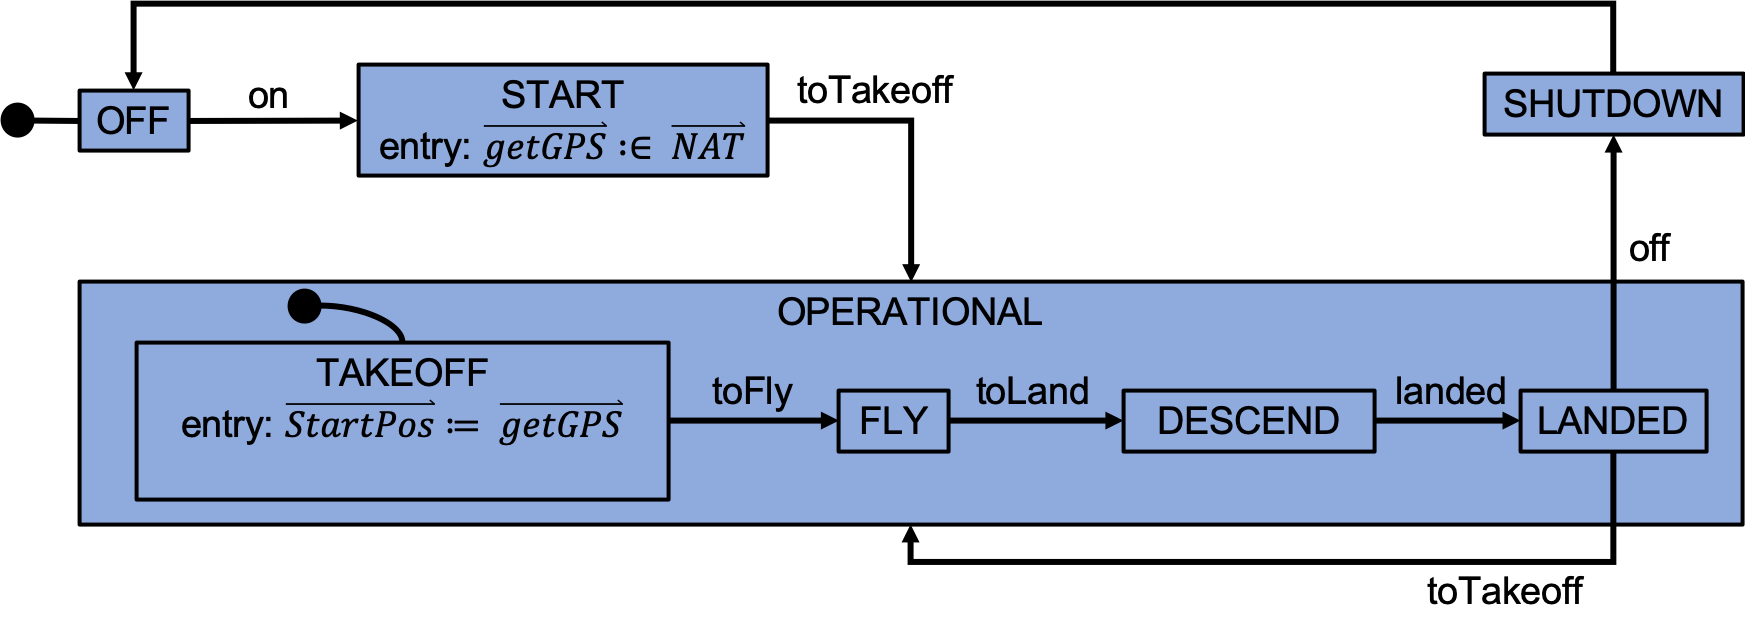
\includegraphics[width=0.95\textwidth]{figures/Picture1.png}
	\caption{Statechart of drone application. Abstract level including only generic behavior. }
	\label{fig:drone1}
	\vspace{-.4cm}
\end{figure} 

Figure~\ref{fig:drone2} shows the first refinement of the model, as we refine the parent state |TAKEOFF|
by introducing child states and new model variables, similar to 
Rule 2 \emph{basic-to-or state rule} defined by Syriani et al.~\SonAdd{\mbox{\cite{Syriani_2019}}}
As part of this refinement we introduced an untriggered transition responsible for 
raising the |toFly| internal trigger, and therefore removed some of the non-determinisms in the abstraction.

\begin{figure}[!h]
	\centering
	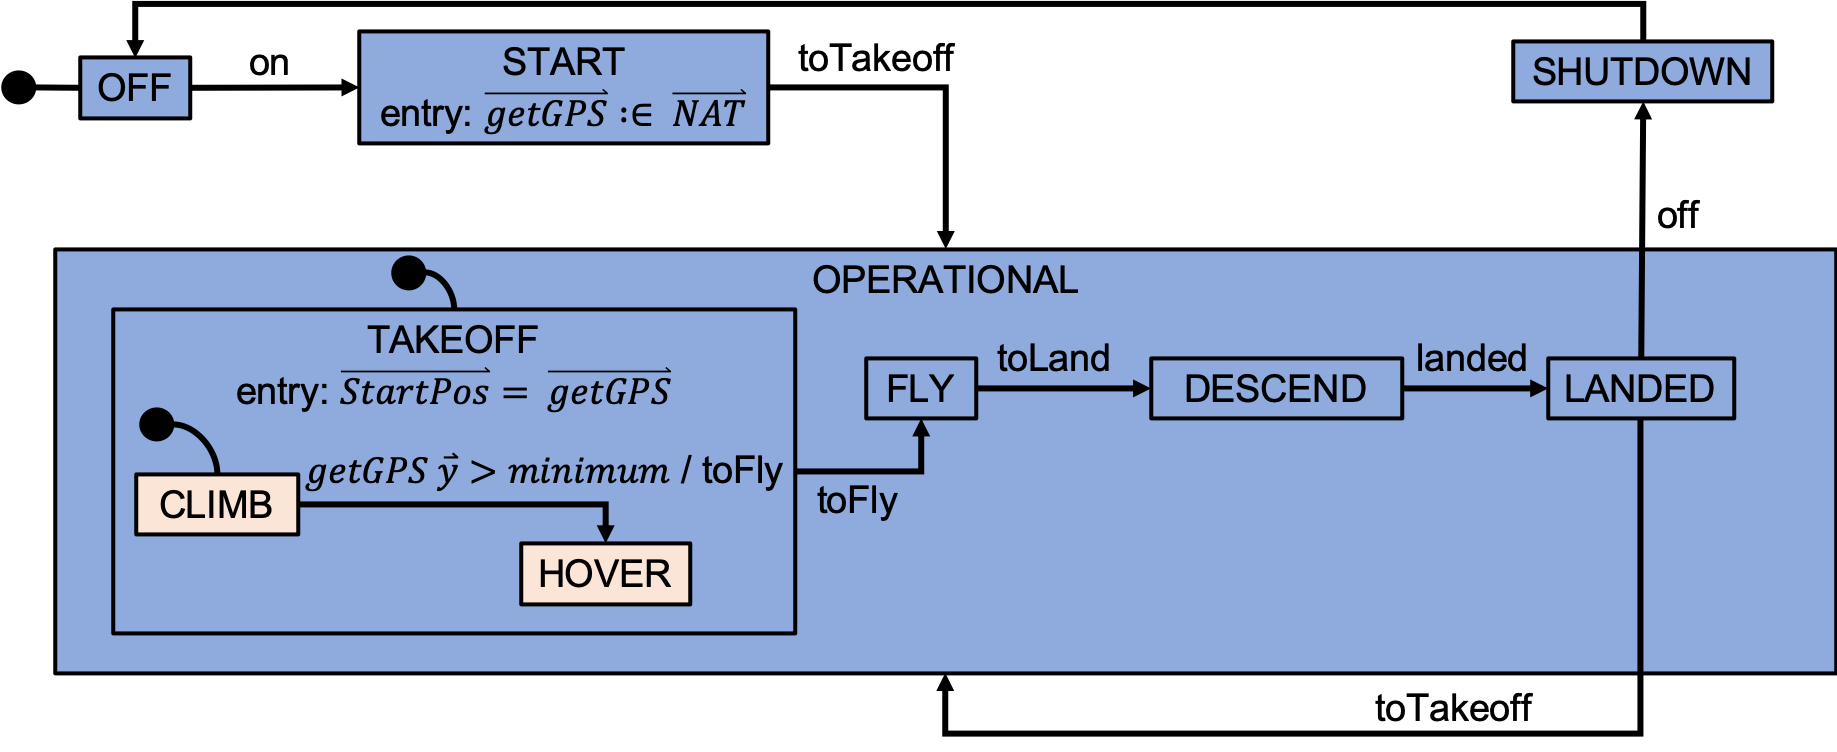
\includegraphics[width=0.95\textwidth]{figures/Picture2.png}
	\caption{Statechart of drone application. Refinement level introducing details for take off.}
	\label{fig:drone2}
\end{figure} 

\begin{figure}[!h]
	\centering
	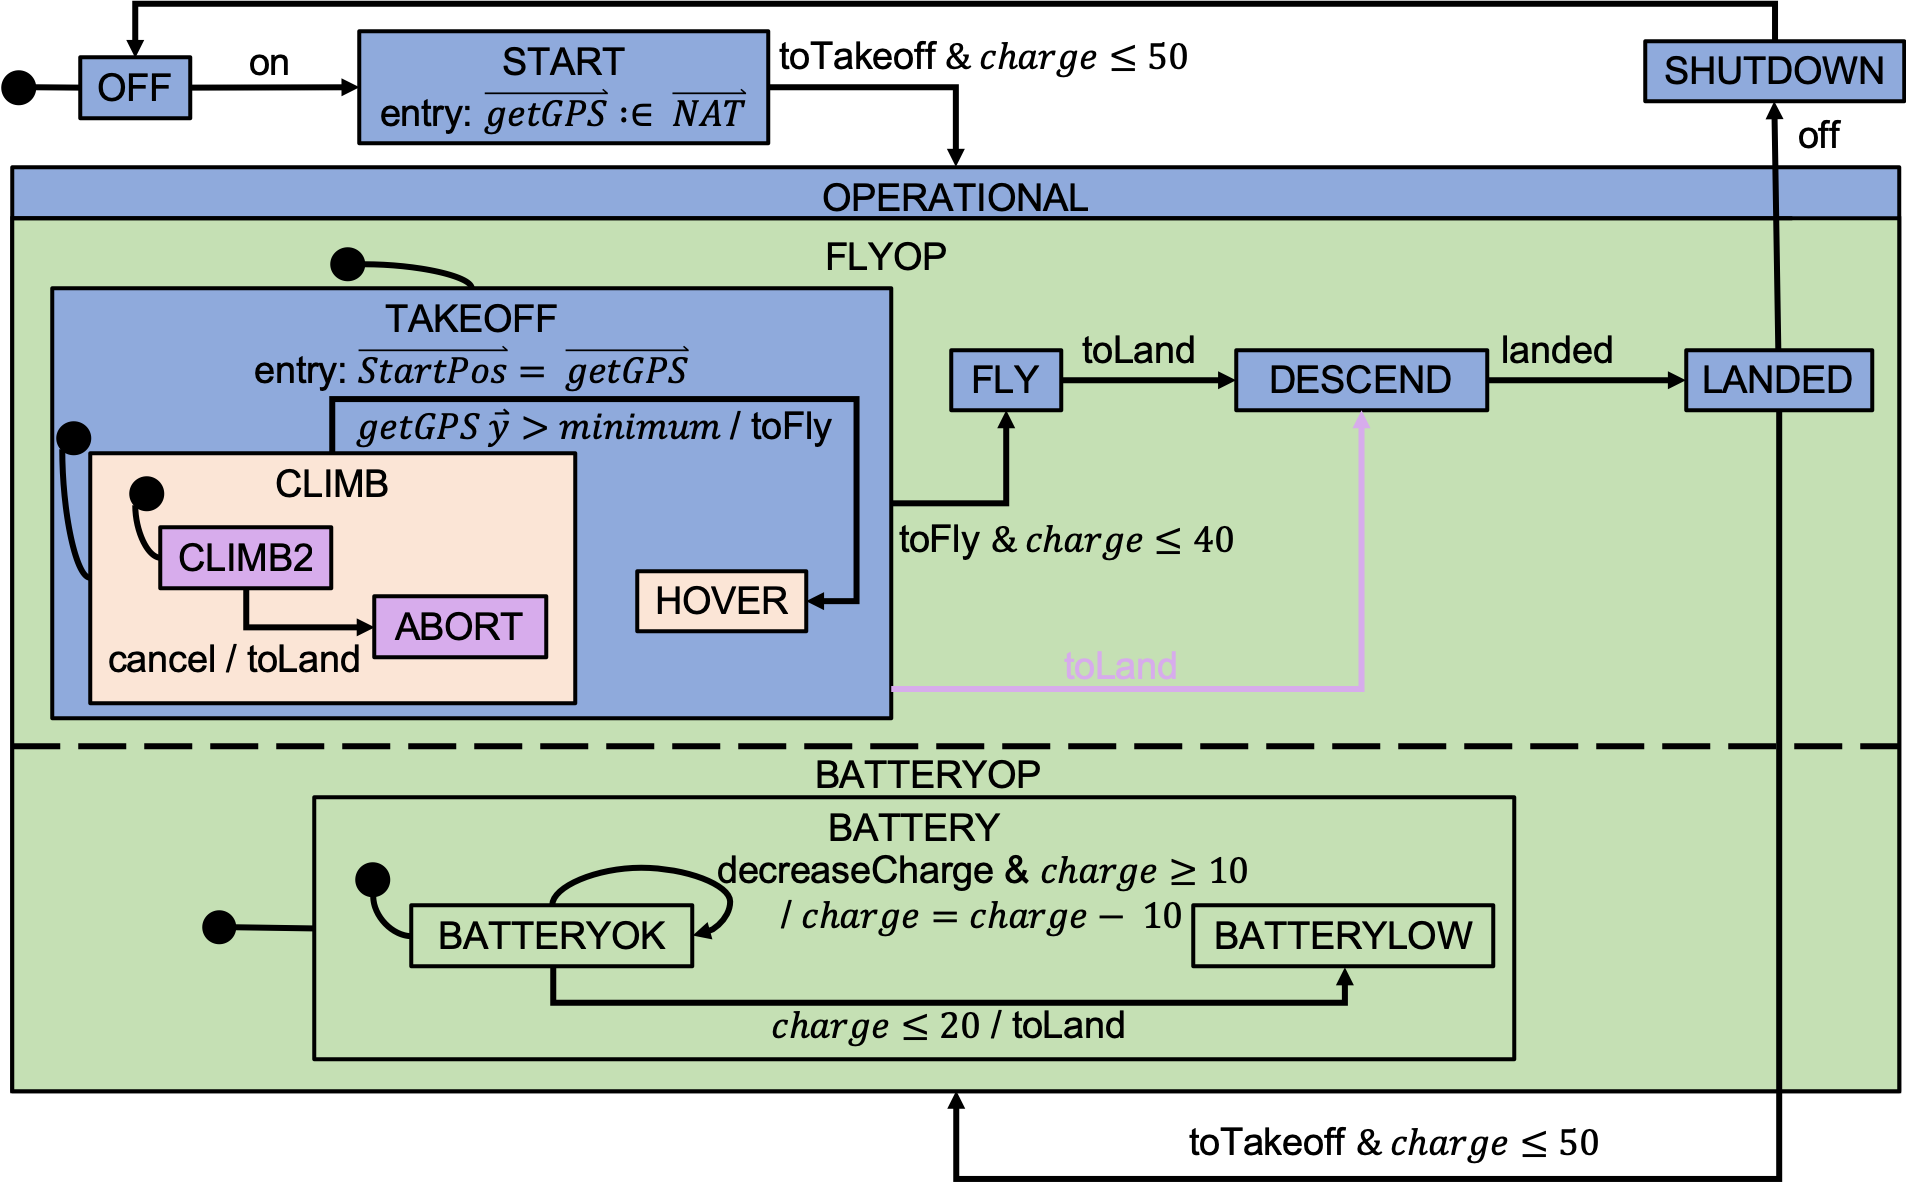
\includegraphics[width=0.95\textwidth]{figures/Picture5.png}
	\caption{Statechart of drone application. 
	Refinement level for battery consumption functionality (shown in green).
	Refinement level for descending capabilities, in case of emergency (shown in lilac).}
	\label{fig:drone4}
\end{figure} 

Figure~\ref{fig:drone4} shows two subsequent refinements to the drone model.
The second refinement, the details of which are shown in green in \SonChange{figure}{Figure}~\ref{fig:drone4}, 
extends the capabilities within |OPERATIONAL| by making it a parallel
state that controls flying and battery related functionality. 
This is the same as Rule 4 \emph{and-state rule} defined by Syriani et al.~\SonAdd{\mbox{\cite{Syriani_2019}}}.
The charge within the drone battery is control by the parallel |BATTERYOP| state. 
The functionality is modeled by introducing a new model variable, |charge|, which is decreased as 
a response to the internal trigger |decreaseCharge|. The aforementioned trigger, is raised non-deterministically by some 
unspecified internal functionality. Our statechart semantics support transition refinement, as such
we are able to modified previously defined transitions. In particular, this type of refinement allow
us to add guards and/or actions to previously defined transitions. The strengthening of guards, or additional 
actions are expressed in term of new model variables that contribute implementation details to the model.
To ensure the drone operates with enough battery power we strengthen the guards of transitions 
to the |FLY| and |TAKEOFF| states.
As part of this design stage we introduce a requirement to constrain drone operation 
to a battery charge of at least 20\% capacity. This can be expressed as
\begin{center}
  |(BATTERYOK = TRUE) => charge > 20|\%\SonAdd{~.}
\end{center}
% \begin{figure}[!h]
% 	\centering
% 	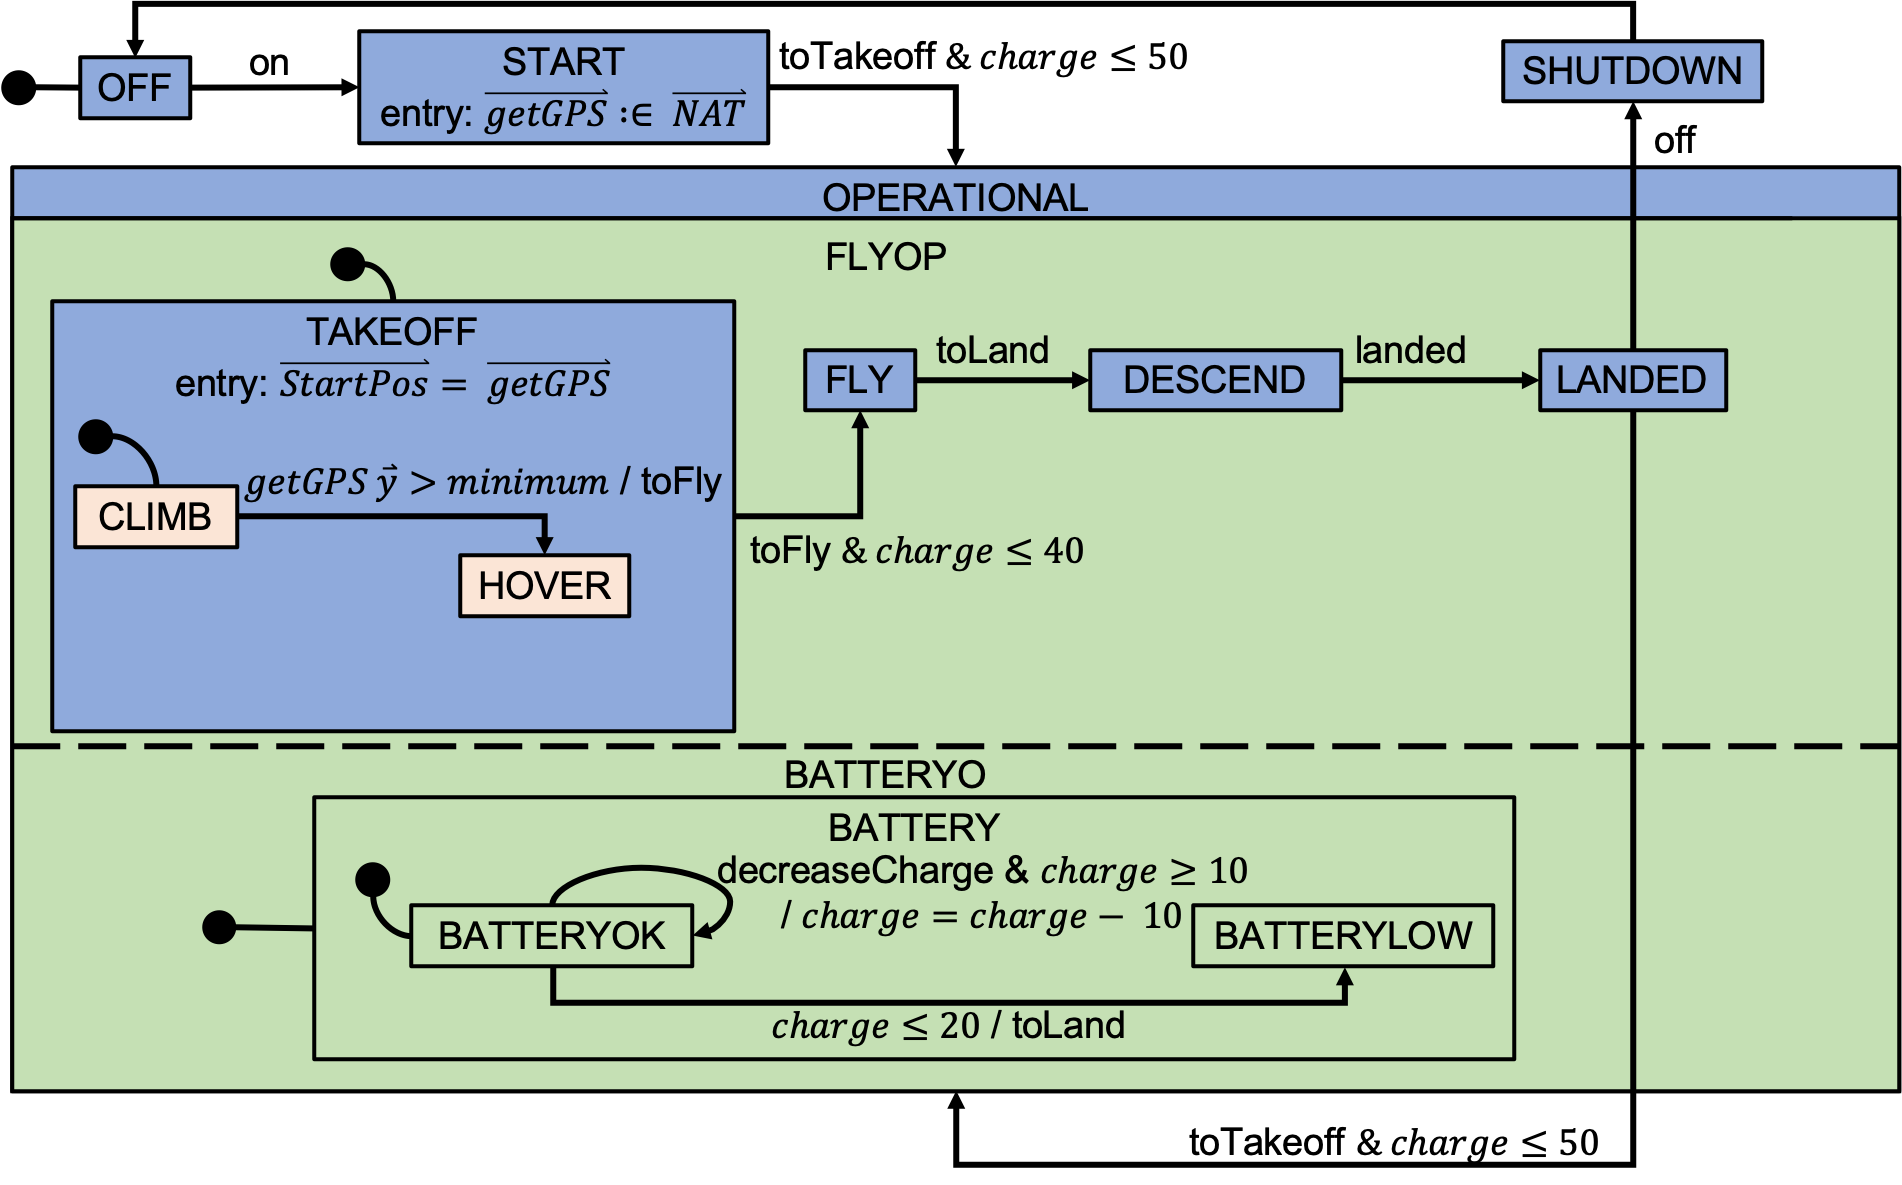
\includegraphics[width=0.95\textwidth]{figures/Picture3.png}
% 	\caption{Statechart of drone application.Refinement level for descending capabilities}
% 	\label{fig:drone3}
% \end{figure} 

Figure~\ref{fig:drone4} shows \SonChange{a}{the} third refinement of the drone model, with features added in lilac.
At this stage we introduce additional implementation details to ensure that under special 
circumstances (e.g. sensing of adverse environment or unexpected battery dropped) the drone is able 
to circumvent flying and proceed to an emergency landing. The previously described requirement can be
expressed as
\begin{center}
  |(TAKEOFF = TRUE) => (BATTERYOK = TRUE ∨ toLand)|~.
\end{center}
To implement this new capability in the design the internal trigger |cancel| is introduced.
The internal trigger |cancel| can be raise non-deterministically by some sensing capability, 
the details of which are not currently implemented. If the trigger is raised the climbing process 
must be aborted and the drone descending sequence shall start. This refinement level is done differently 
from Syriani et al.~\cite{Syriani_2019}, which follows Rule 7 \emph{state extension rule}. 
The aforementioned rule requires a data remapping of the abstract states |TAKEOFF|, |CLIMB| and |HOVER|,
which should be distinct from the states in this refinement, as the state |ABORT| is introduced.
In contrast, we implement this refinement using a rule similar to Syriani et al.'s 
Rule 2 \emph{basic-to-or state rule}, which introduces the concrete states |CLIMB2| and |ABORT| 
to the abstract state |CLIMB|.


% Syriani et al. refinement rules
% Rule 1 \emph{action rule}
% Rule 2 \emph{basic-to-or state rule}
% Rule 3 \emph{or-to-and state rule}
% Rule 4 \emph{and-state rule}
% Rule 5 \emph{transition rule}
% Rule 6 \emph{fork rule}
% Rule 7 \emph{state extension rule}
% Rule 8 \emph{path refinement rule}

% Event-B refinement rules
% https://www3.hhu.de/stups/handbook/rodin/current/html/generated_proof_obligations.html
% guard strengthening
% action simulation
% equality of a preserved variable
% guard strengthening (merge)
% well definedness of a witness
% feasibility of witness
% decreasing of variant

%%% Local Variables:
%%% mode: latex
%%% TeX-master: "../main"
%%% End:
